% Options for packages loaded elsewhere
\PassOptionsToPackage{unicode}{hyperref}
\PassOptionsToPackage{hyphens}{url}
%
\documentclass[
]{book}
\usepackage{amsmath,amssymb}
\usepackage{lmodern}
\usepackage{iftex}
\ifPDFTeX
  \usepackage[T1]{fontenc}
  \usepackage[utf8]{inputenc}
  \usepackage{textcomp} % provide euro and other symbols
\else % if luatex or xetex
  \usepackage{unicode-math}
  \defaultfontfeatures{Scale=MatchLowercase}
  \defaultfontfeatures[\rmfamily]{Ligatures=TeX,Scale=1}
\fi
% Use upquote if available, for straight quotes in verbatim environments
\IfFileExists{upquote.sty}{\usepackage{upquote}}{}
\IfFileExists{microtype.sty}{% use microtype if available
  \usepackage[]{microtype}
  \UseMicrotypeSet[protrusion]{basicmath} % disable protrusion for tt fonts
}{}
\makeatletter
\@ifundefined{KOMAClassName}{% if non-KOMA class
  \IfFileExists{parskip.sty}{%
    \usepackage{parskip}
  }{% else
    \setlength{\parindent}{0pt}
    \setlength{\parskip}{6pt plus 2pt minus 1pt}}
}{% if KOMA class
  \KOMAoptions{parskip=half}}
\makeatother
\usepackage{xcolor}
\IfFileExists{xurl.sty}{\usepackage{xurl}}{} % add URL line breaks if available
\IfFileExists{bookmark.sty}{\usepackage{bookmark}}{\usepackage{hyperref}}
\hypersetup{
  pdftitle={Diplomado de Econometría Financiera},
  pdfauthor={Benjamin Oliva y Emiliano Pérez Caullieres},
  hidelinks,
  pdfcreator={LaTeX via pandoc}}
\urlstyle{same} % disable monospaced font for URLs
\usepackage{color}
\usepackage{fancyvrb}
\newcommand{\VerbBar}{|}
\newcommand{\VERB}{\Verb[commandchars=\\\{\}]}
\DefineVerbatimEnvironment{Highlighting}{Verbatim}{commandchars=\\\{\}}
% Add ',fontsize=\small' for more characters per line
\usepackage{framed}
\definecolor{shadecolor}{RGB}{248,248,248}
\newenvironment{Shaded}{\begin{snugshade}}{\end{snugshade}}
\newcommand{\AlertTok}[1]{\textcolor[rgb]{0.94,0.16,0.16}{#1}}
\newcommand{\AnnotationTok}[1]{\textcolor[rgb]{0.56,0.35,0.01}{\textbf{\textit{#1}}}}
\newcommand{\AttributeTok}[1]{\textcolor[rgb]{0.77,0.63,0.00}{#1}}
\newcommand{\BaseNTok}[1]{\textcolor[rgb]{0.00,0.00,0.81}{#1}}
\newcommand{\BuiltInTok}[1]{#1}
\newcommand{\CharTok}[1]{\textcolor[rgb]{0.31,0.60,0.02}{#1}}
\newcommand{\CommentTok}[1]{\textcolor[rgb]{0.56,0.35,0.01}{\textit{#1}}}
\newcommand{\CommentVarTok}[1]{\textcolor[rgb]{0.56,0.35,0.01}{\textbf{\textit{#1}}}}
\newcommand{\ConstantTok}[1]{\textcolor[rgb]{0.00,0.00,0.00}{#1}}
\newcommand{\ControlFlowTok}[1]{\textcolor[rgb]{0.13,0.29,0.53}{\textbf{#1}}}
\newcommand{\DataTypeTok}[1]{\textcolor[rgb]{0.13,0.29,0.53}{#1}}
\newcommand{\DecValTok}[1]{\textcolor[rgb]{0.00,0.00,0.81}{#1}}
\newcommand{\DocumentationTok}[1]{\textcolor[rgb]{0.56,0.35,0.01}{\textbf{\textit{#1}}}}
\newcommand{\ErrorTok}[1]{\textcolor[rgb]{0.64,0.00,0.00}{\textbf{#1}}}
\newcommand{\ExtensionTok}[1]{#1}
\newcommand{\FloatTok}[1]{\textcolor[rgb]{0.00,0.00,0.81}{#1}}
\newcommand{\FunctionTok}[1]{\textcolor[rgb]{0.00,0.00,0.00}{#1}}
\newcommand{\ImportTok}[1]{#1}
\newcommand{\InformationTok}[1]{\textcolor[rgb]{0.56,0.35,0.01}{\textbf{\textit{#1}}}}
\newcommand{\KeywordTok}[1]{\textcolor[rgb]{0.13,0.29,0.53}{\textbf{#1}}}
\newcommand{\NormalTok}[1]{#1}
\newcommand{\OperatorTok}[1]{\textcolor[rgb]{0.81,0.36,0.00}{\textbf{#1}}}
\newcommand{\OtherTok}[1]{\textcolor[rgb]{0.56,0.35,0.01}{#1}}
\newcommand{\PreprocessorTok}[1]{\textcolor[rgb]{0.56,0.35,0.01}{\textit{#1}}}
\newcommand{\RegionMarkerTok}[1]{#1}
\newcommand{\SpecialCharTok}[1]{\textcolor[rgb]{0.00,0.00,0.00}{#1}}
\newcommand{\SpecialStringTok}[1]{\textcolor[rgb]{0.31,0.60,0.02}{#1}}
\newcommand{\StringTok}[1]{\textcolor[rgb]{0.31,0.60,0.02}{#1}}
\newcommand{\VariableTok}[1]{\textcolor[rgb]{0.00,0.00,0.00}{#1}}
\newcommand{\VerbatimStringTok}[1]{\textcolor[rgb]{0.31,0.60,0.02}{#1}}
\newcommand{\WarningTok}[1]{\textcolor[rgb]{0.56,0.35,0.01}{\textbf{\textit{#1}}}}
\usepackage{longtable,booktabs,array}
\usepackage{calc} % for calculating minipage widths
% Correct order of tables after \paragraph or \subparagraph
\usepackage{etoolbox}
\makeatletter
\patchcmd\longtable{\par}{\if@noskipsec\mbox{}\fi\par}{}{}
\makeatother
% Allow footnotes in longtable head/foot
\IfFileExists{footnotehyper.sty}{\usepackage{footnotehyper}}{\usepackage{footnote}}
\makesavenoteenv{longtable}
\usepackage{graphicx}
\makeatletter
\def\maxwidth{\ifdim\Gin@nat@width>\linewidth\linewidth\else\Gin@nat@width\fi}
\def\maxheight{\ifdim\Gin@nat@height>\textheight\textheight\else\Gin@nat@height\fi}
\makeatother
% Scale images if necessary, so that they will not overflow the page
% margins by default, and it is still possible to overwrite the defaults
% using explicit options in \includegraphics[width, height, ...]{}
\setkeys{Gin}{width=\maxwidth,height=\maxheight,keepaspectratio}
% Set default figure placement to htbp
\makeatletter
\def\fps@figure{htbp}
\makeatother
\setlength{\emergencystretch}{3em} % prevent overfull lines
\providecommand{\tightlist}{%
  \setlength{\itemsep}{0pt}\setlength{\parskip}{0pt}}
\setcounter{secnumdepth}{5}
\usepackage{booktabs}
\ifLuaTeX
  \usepackage{selnolig}  % disable illegal ligatures
\fi
\usepackage[]{natbib}
\bibliographystyle{apalike}

\title{Diplomado de Econometría Financiera}
\author{Benjamin Oliva y Emiliano Pérez Caullieres}
\date{2022-09-06}

\begin{document}
\maketitle

{
\setcounter{tocdepth}{1}
\tableofcontents
}
\hypertarget{muxednimos-cuadrados-ordinarios}{%
\chapter{Mínimos Cuadrados Ordinarios}\label{muxednimos-cuadrados-ordinarios}}

\hypertarget{el-problema}{%
\section{El problema}\label{el-problema}}

Recordando que el método de MCO resulta en encontrar la combinación de valores de los estimadores de los parámetros \(\hat{\boldsymbol{\beta}}\) que permita minimizar la suma de los residuales (estimadores de los términos de erro \(\boldsymbol{\varepsilon}\)) al cuadrado dada por:

\[
    \sum^{N}_{i=1}{e^2_i} = \sum^{N}_{i = 1}{(y_i - \mathbf{X}'_i \hat{\boldsymbol{\beta}})^2}
\]

Donde \(\hat{\boldsymbol{\beta}}\) denota el vector de estimadores \(\hat{\beta}_1, \ldots, \hat{\beta}_K\) y dado que \((e_1, e_2, \ldots, e_n)'(e_1, e_2, \ldots, e_n) = {\mathbf{e'e}}\), el problema del método de MCO consiste en resolver el problema de óptimización:

\begin{eqnarray*}
Minimizar_{\hat{\boldsymbol \beta}} S(\hat{\boldsymbol \beta})  =  Minimizar_{\hat{\boldsymbol \beta}} \mathbf{e'e} \\
    =  Minimizar_{\hat{\boldsymbol \beta}} (\mathbf{Y}-\mathbf{X}\hat{\boldsymbol \beta})'(\mathbf{Y}-\mathbf{X}\hat{\boldsymbol \beta})
\end{eqnarray*}

Expandiendo la expresión \(\mathbf{e'e}\) obtenemos:
\[
    \mathbf{e'e} = \mathbf{Y'Y} - 2 \mathbf{Y'X} \hat{\boldsymbol \beta} + \hat{\boldsymbol \beta}' \mathbf{X'X}\hat{\boldsymbol \beta}
\]

De esta forma obtenemos que las condiciones necesarias de un mínimo son:

\[
    \frac{\partial S(\hat{\boldsymbol \beta})}{\partial \hat{\boldsymbol \beta}} = -2{\mathbf{X'Y}} + 2{\mathbf{X'X}} \hat{\boldsymbol{\beta}} = \mathbf{0}
\]
Y se pueden despejar las \textit{ecuaciones normales} dadas por:

Debido a que el objetivo es encontrar la matriz \(\hat{\boldsymbol\beta}\) despejamos:

\[\hat{\boldsymbol \beta} = (\mathbf{X'X})^{-1}\mathbf{X'Y}
\]
\[
    \mathbf{X'X}\hat{\boldsymbol \beta} = \mathbf{X'Y}
\]

\hypertarget{estimaciuxf3n-r}{%
\section{Estimación R}\label{estimaciuxf3n-r}}

Para la estimación utilizaremos el paquete ``BatchGetSymbols''. Este paquete nos permitirá descargar información acerca de la bolsa de valores internacional.

\hypertarget{dependencias}{%
\subsection{Dependencias}\label{dependencias}}

\begin{Shaded}
\begin{Highlighting}[]
\CommentTok{\#install.packages("pacman")}
\CommentTok{\#pacman nos permite cargar varias librerias en una sola línea}
\FunctionTok{library}\NormalTok{(pacman)}
\NormalTok{pacman}\SpecialCharTok{::}\FunctionTok{p\_load}\NormalTok{(tidyverse,BatchGetSymbols,ggplot2, lubridate)}
\end{Highlighting}
\end{Shaded}

\hypertarget{descarga-de-los-valores}{%
\subsection{Descarga de los valores}\label{descarga-de-los-valores}}

\begin{Shaded}
\begin{Highlighting}[]
\CommentTok{\#Primero determinamos el lapso de tiempo}
\NormalTok{pd}\OtherTok{\textless{}{-}}\FunctionTok{Sys.Date}\NormalTok{()}\SpecialCharTok{{-}}\DecValTok{365} \CommentTok{\#primer fecha}
\NormalTok{pd}
\CommentTok{\#\textgreater{} [1] "2021{-}09{-}06"}
\NormalTok{ld}\OtherTok{\textless{}{-}}\FunctionTok{Sys.Date}\NormalTok{() }\CommentTok{\#última fecha}
\NormalTok{ld}
\CommentTok{\#\textgreater{} [1] "2022{-}09{-}06"}
\CommentTok{\#Intervalos de tiempo}
\NormalTok{int}\OtherTok{\textless{}{-}}\StringTok{"monthly"}
\CommentTok{\#Datos a elegir}
\NormalTok{dt}\OtherTok{\textless{}{-}}\FunctionTok{c}\NormalTok{(}\StringTok{"AMZN"}\NormalTok{)}

\CommentTok{\#Descargando los valores}
\NormalTok{?}\FunctionTok{BatchGetSymbols}\NormalTok{()}
\NormalTok{data}\OtherTok{\textless{}{-}} \FunctionTok{BatchGetSymbols}\NormalTok{(}\AttributeTok{tickers =}\NormalTok{ dt,}
                       \AttributeTok{first.date =}\NormalTok{ pd,}
                       \AttributeTok{last.date =}\NormalTok{ ld,}
                       \AttributeTok{freq.data =}\NormalTok{ int,}
                       \AttributeTok{do.cache =} \ConstantTok{FALSE}\NormalTok{,}
                       \AttributeTok{thresh.bad.data =} \DecValTok{0}\NormalTok{)}

\CommentTok{\#Generando data frame con los valores}
\NormalTok{data\_precio}\OtherTok{\textless{}{-}}\NormalTok{data}\SpecialCharTok{$}\NormalTok{df.tickers}
\FunctionTok{colnames}\NormalTok{(data\_precio)}
\CommentTok{\#\textgreater{}  [1] "ticker"              "ref.date"           }
\CommentTok{\#\textgreater{}  [3] "volume"              "price.open"         }
\CommentTok{\#\textgreater{}  [5] "price.high"          "price.low"          }
\CommentTok{\#\textgreater{}  [7] "price.close"         "price.adjusted"     }
\CommentTok{\#\textgreater{}  [9] "ret.adjusted.prices" "ret.closing.prices"}
\end{Highlighting}
\end{Shaded}

\hypertarget{gruxe1ficas}{%
\subsection{Gráficas}\label{gruxe1ficas}}

\begin{Shaded}
\begin{Highlighting}[]
\NormalTok{sp\_precio}\OtherTok{\textless{}{-}}\FunctionTok{ggplot}\NormalTok{(data\_precio, }\FunctionTok{aes}\NormalTok{(}\AttributeTok{x=}\NormalTok{ref.date, }\AttributeTok{y=}\NormalTok{price.open))}\SpecialCharTok{+}\FunctionTok{geom\_point}\NormalTok{(}\AttributeTok{size =}\DecValTok{2}\NormalTok{, }\AttributeTok{colour =} \StringTok{"black"}\NormalTok{)}\SpecialCharTok{+}\FunctionTok{labs}\NormalTok{(}\AttributeTok{x=}\StringTok{"Fecha"}\NormalTok{, }\AttributeTok{y=}\StringTok{"Precio de apertura (USD)"}\NormalTok{, }\AttributeTok{title=}\StringTok{"Precio de apertura de AMZN en el ultimo año"}\NormalTok{)}\SpecialCharTok{+} \FunctionTok{theme\_light}\NormalTok{()}\SpecialCharTok{+} \FunctionTok{geom\_smooth}\NormalTok{(}\AttributeTok{method =}\NormalTok{ lm, }\AttributeTok{se =} \ConstantTok{TRUE}\NormalTok{)}
\NormalTok{sp\_precio}
\end{Highlighting}
\end{Shaded}

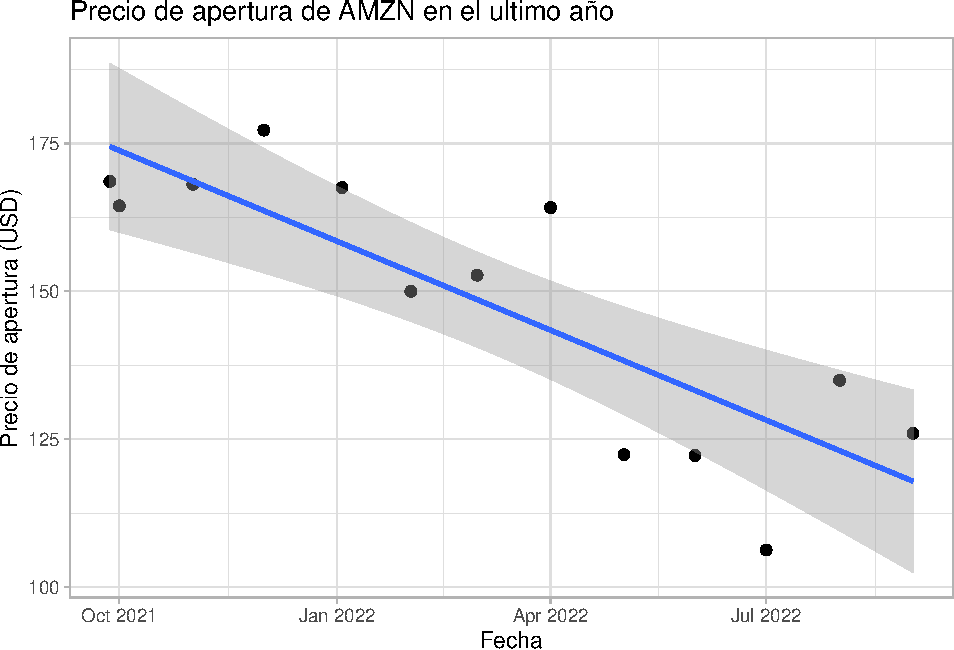
\includegraphics{index_files/figure-latex/unnamed-chunk-3-1.pdf}

\begin{Shaded}
\begin{Highlighting}[]

\NormalTok{sp\_volumen}\OtherTok{\textless{}{-}}\FunctionTok{ggplot}\NormalTok{(data\_precio, }\FunctionTok{aes}\NormalTok{(}\AttributeTok{x=}\NormalTok{ref.date, }\AttributeTok{y=}\NormalTok{volume))}\SpecialCharTok{+}\FunctionTok{geom\_point}\NormalTok{(}\AttributeTok{size =}\DecValTok{2}\NormalTok{, }\AttributeTok{colour =} \StringTok{"black"}\NormalTok{)}\SpecialCharTok{+}\FunctionTok{labs}\NormalTok{(}\AttributeTok{x=}\StringTok{"Fecha"}\NormalTok{, }\AttributeTok{y=}\StringTok{"Volumen"}\NormalTok{, }\AttributeTok{title=}\StringTok{"Volumenes de AMZN en el ultimo año"}\NormalTok{)}\SpecialCharTok{+} \FunctionTok{theme\_light}\NormalTok{()}\SpecialCharTok{+} \FunctionTok{geom\_smooth}\NormalTok{(}\AttributeTok{method =}\NormalTok{ lm, }\AttributeTok{se =} \ConstantTok{TRUE}\NormalTok{)}
\NormalTok{sp\_volumen}
\end{Highlighting}
\end{Shaded}

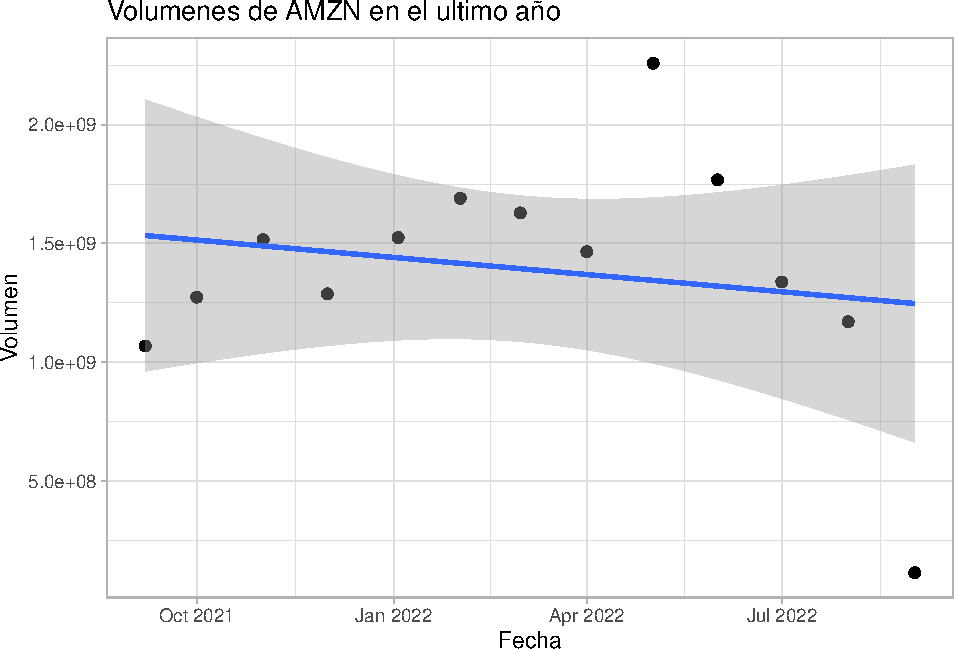
\includegraphics{index_files/figure-latex/unnamed-chunk-3-2.pdf}

\hypertarget{regresiuxf3n-lineal-que-optiene-los-coeficientes-hatboldsymbol-beta}{%
\subsection{\texorpdfstring{Regresión lineal que optiene los coeficientes \(\hat{\boldsymbol \beta}\)}{Regresión lineal que optiene los coeficientes \textbackslash hat\{\textbackslash boldsymbol \textbackslash beta\}}}\label{regresiuxf3n-lineal-que-optiene-los-coeficientes-hatboldsymbol-beta}}

\begin{Shaded}
\begin{Highlighting}[]
\CommentTok{\#datos estadísticos}
\FunctionTok{summary}\NormalTok{(data\_precio[}\FunctionTok{c}\NormalTok{(}\StringTok{"price.open"}\NormalTok{,}\StringTok{"volume"}\NormalTok{)])}
\CommentTok{\#\textgreater{}    price.open        volume         }
\CommentTok{\#\textgreater{}  Min.   :106.3   Min.   :1.140e+08  }
\CommentTok{\#\textgreater{}  1st Qu.:126.0   1st Qu.:1.273e+09  }
\CommentTok{\#\textgreater{}  Median :152.7   Median :1.465e+09  }
\CommentTok{\#\textgreater{}  Mean   :148.5   Mean   :1.392e+09  }
\CommentTok{\#\textgreater{}  3rd Qu.:167.6   3rd Qu.:1.628e+09  }
\CommentTok{\#\textgreater{}  Max.   :177.2   Max.   :2.258e+09}
\CommentTok{\#análisis de regresión lineal lm() y=precio,x=fecha}
\NormalTok{reg\_tiempo\_precio}\OtherTok{\textless{}{-}}\FunctionTok{lm}\NormalTok{(price.open}\SpecialCharTok{\textasciitilde{}}\NormalTok{ref.date, }\AttributeTok{data=}\NormalTok{data\_precio) }
\CommentTok{\#¡Siempre se pone dentro de lm() la variable dependiente primero y luego la independiete!}
\FunctionTok{summary}\NormalTok{(reg\_tiempo\_precio)}
\CommentTok{\#\textgreater{} }
\CommentTok{\#\textgreater{} Call:}
\CommentTok{\#\textgreater{} lm(formula = price.open \textasciitilde{} ref.date, data = data\_precio)}
\CommentTok{\#\textgreater{} }
\CommentTok{\#\textgreater{} Residuals:}
\CommentTok{\#\textgreater{}      Min       1Q   Median       3Q      Max }
\CommentTok{\#\textgreater{} {-}21.9379  {-}9.7257  {-}0.8686   9.1948  20.6055 }
\CommentTok{\#\textgreater{} }
\CommentTok{\#\textgreater{} Coefficients:}
\CommentTok{\#\textgreater{}               Estimate Std. Error t value Pr(\textgreater{}|t|)    }
\CommentTok{\#\textgreater{} (Intercept) 3355.37814  615.12157   5.455 0.000199 ***}
\CommentTok{\#\textgreater{} ref.date      {-}0.16831    0.03228  {-}5.214 0.000288 ***}
\CommentTok{\#\textgreater{} {-}{-}{-}}
\CommentTok{\#\textgreater{} Signif. codes:  }
\CommentTok{\#\textgreater{} 0 \textquotesingle{}***\textquotesingle{} 0.001 \textquotesingle{}**\textquotesingle{} 0.01 \textquotesingle{}*\textquotesingle{} 0.05 \textquotesingle{}.\textquotesingle{} 0.1 \textquotesingle{} \textquotesingle{} 1}
\CommentTok{\#\textgreater{} }
\CommentTok{\#\textgreater{} Residual standard error: 13.13 on 11 degrees of freedom}
\CommentTok{\#\textgreater{} Multiple R{-}squared:  0.7119, Adjusted R{-}squared:  0.6857 }
\CommentTok{\#\textgreater{} F{-}statistic: 27.18 on 1 and 11 DF,  p{-}value: 0.0002884}

\CommentTok{\#análisis de regresión lineal lm() y=volumen,x=fecha}
\NormalTok{reg\_tiempo\_volumen}\OtherTok{\textless{}{-}}\FunctionTok{lm}\NormalTok{(volume}\SpecialCharTok{\textasciitilde{}}\NormalTok{ref.date, }\AttributeTok{data=}\NormalTok{data\_precio)}
\FunctionTok{summary}\NormalTok{(reg\_tiempo\_volumen)}
\CommentTok{\#\textgreater{} }
\CommentTok{\#\textgreater{} Call:}
\CommentTok{\#\textgreater{} lm(formula = volume \textasciitilde{} ref.date, data = data\_precio)}
\CommentTok{\#\textgreater{} }
\CommentTok{\#\textgreater{} Residuals:}
\CommentTok{\#\textgreater{}        Min         1Q     Median         3Q        Max }
\CommentTok{\#\textgreater{} {-}1.133e+09 {-}1.780e+08  4.137e+07  2.347e+08  9.141e+08 }
\CommentTok{\#\textgreater{} }
\CommentTok{\#\textgreater{} Coefficients:}
\CommentTok{\#\textgreater{}               Estimate Std. Error t value Pr(\textgreater{}|t|)}
\CommentTok{\#\textgreater{} (Intercept)  1.659e+10  2.358e+10   0.704    0.496}
\CommentTok{\#\textgreater{} ref.date    {-}7.978e+05  1.237e+06  {-}0.645    0.532}
\CommentTok{\#\textgreater{} }
\CommentTok{\#\textgreater{} Residual standard error: 503100000 on 11 degrees of freedom}
\CommentTok{\#\textgreater{} Multiple R{-}squared:  0.03641,    Adjusted R{-}squared:  {-}0.05119 }
\CommentTok{\#\textgreater{} F{-}statistic: 0.4157 on 1 and 11 DF,  p{-}value: 0.5323}
\end{Highlighting}
\end{Shaded}

\hypertarget{ejercicio}{%
\section{Ejercicio}\label{ejercicio}}

El objetivo de este ejrcicio es simplemente que indiquen y modifiquen los errores en el código. Así pues, deberán descomentar \emph{-quitar las \#antes del código-} para empezar el ejercicio.

\hypertarget{section}{%
\subsection{1}\label{section}}

El objetivo de este código es explicar la variable \textbf{``volume''} con la variable \textbf{``price.high''}.

\begin{Shaded}
\begin{Highlighting}[]
\CommentTok{\#reg\_tiempo\_ej1\textless{}{-}lm(price.high\textasciitilde{}volume, data=data\_precio)}
\CommentTok{\#sumary(reg\_tiempo\_ej1)}
\end{Highlighting}
\end{Shaded}

\hypertarget{section-1}{%
\subsection{2}\label{section-1}}

El objetivo de este código es explicar la variable \textbf{``volume''} con la variable \textbf{``price.low''}.

\begin{Shaded}
\begin{Highlighting}[]
\CommentTok{\#reg\_tiempo\_ej2\textless{}{-}lm(price.low\textasciitilde{}volume, data=data\_precio)}
\CommentTok{\#summary(reg\_tiempo\_ej1)}
\end{Highlighting}
\end{Shaded}

\hypertarget{opcional}{%
\subsection{3 (opcional)}\label{opcional}}

El objetivo de este ejercicio es descargar los valores del stock de Tesla \emph{BMV: TSLA} en los últimos \emph{dos años}.

\begin{Shaded}
\begin{Highlighting}[]
\CommentTok{\#dt\_ej3\textless{}{-}("TSLA")}
\CommentTok{\#pdej\textless{}{-}Sys.Date(){-}(365*3) \#primer fecha}
\CommentTok{\#pdej}
\CommentTok{\#Descargando los valores}
\CommentTok{\#dataej3\textless{}{-} BatchgetSymbols(tickers = dt\_ej3,}
                       \CommentTok{\#first.date = pdej,}
                       \CommentTok{\#last.date = ld,}
                       \CommentTok{\#freq.data = int,}
                       \CommentTok{\#do.cache = FALSE,}
                       \CommentTok{\#thresh.bad.data = 0)}

\CommentTok{\#Generando data frame con los valores}
\CommentTok{\#data\_precio\_ej2\textless{}{-}dataej3$df.tickers}
\CommentTok{\#1colnames(data\_precio\_ej2)}
\end{Highlighting}
\end{Shaded}

\hypertarget{muxe1xima-verosimilitud}{%
\chapter{Máxima Verosimilitud}\label{muxe1xima-verosimilitud}}

\hypertarget{el-problema-1}{%
\section{El problema}\label{el-problema-1}}

Recordemos que dado \(f(y_i | \mathbf{x}_i)\) la función de densidad condicional de \(y_i\) dado \(\mathbf{x}_i\). Sea \(\boldsymbol{\theta}\) un conjunto de parámetros de la función. Entonces la función de densidad conjunta de variables aleatorias independientes \(\{ y_i : y_i \in \mathbb{R} \}\) dados los valores \(\{ \mathbf{x}_i : \mathbf{x}_i \in \mathbb{R}^K \}\) estará dada por:

\begin{equation}
    \Pi_{i = 1}^{n} f(y_i | \mathbf{x}_i; \boldsymbol{\theta}) = f(y_1, y_2, \ldots, y_n | \mathbf{x}_1, \mathbf{x}_2, \ldots, \mathbf{x}_n; \boldsymbol{\theta}) = L(\boldsymbol{\theta})
    \label{eq:EqLikehood}
\end{equation}

A la ecuación \eqref{eq:EqLikehood} se le conoce como ecuación de verosimilitud. El problema de máxima verosimilitud entonces será:
\begin{equation}
    \max_{\boldsymbol{\theta} \in \boldsymbol{\Theta}} \Pi_{i = 1}^{n} f(y_i | \mathbf{x}_i; \boldsymbol{\theta}) = \max_{\boldsymbol{\theta} \in \boldsymbol{\Theta}} L(\boldsymbol{\theta})
        \label{eq:EqMaxLike}
\end{equation}

Dado que el logaritmo natural es una transformación monotona, podemos decir que el problema de la ecuación \eqref{eq:EqMaxLike} es equivalente a:

\begin{equation}
     \max_{\boldsymbol{\theta} \in \boldsymbol{\Theta}} ln L(\boldsymbol{\theta}) = \max_{\boldsymbol{\theta} \in \boldsymbol{\Theta}} ln \Pi_{i = 1}^{n} f(y_i | \mathbf{x}_i; \boldsymbol{\theta}) = \max_{\boldsymbol{\theta} \in \boldsymbol{\Theta}} \sum_{i = 1}^{n} ln f(y_i | \mathbf{x}_i; \boldsymbol{\theta})
            \label{eq:EqLogML}
\end{equation}

Para solucionnar el problema se tiene que determinar las condicones de primer y segundo orden, las cuales serán:
\begin{equation}
    \frac{\partial}{\partial \boldsymbol{\theta}} ln L(\boldsymbol{\theta}) = \nabla ln L(\boldsymbol{\theta})
          \label{eq:MLCPO}
\end{equation}

\begin{equation}
    \frac{\partial^2}{\partial^2 \boldsymbol{\theta}} ln L(\boldsymbol{\theta}) = \frac{\partial}{\partial \boldsymbol{\theta}} ln L(\boldsymbol{\theta}) \cdot  \frac{\partial}{\partial \boldsymbol{\theta}} ln L(\boldsymbol{\theta}') = H(\boldsymbol{\theta})
             \label{eq:MLCSO}
\end{equation}

La solución estará dada por aquel valor de \(\hat{\boldsymbol{\theta}}\) que hace:
\begin{equation*}
    \frac{\partial}{\partial \boldsymbol{\theta}} ln L(\hat{\boldsymbol{\theta}}) = 0
\end{equation*}

A su vez, la varianza será aquella que resulta de:
\begin{equation*}
    Var[\hat{\boldsymbol{\theta}} | \mathbf{X}] = \left( - \mathbb{E}_{\hat{\boldsymbol{\theta}}}[H(\boldsymbol{\theta})] \right)^{-1}
\end{equation*}

\hypertarget{estimaciuxf3n-y-simunlaciuxf3n}{%
\section{Estimación y simunlación}\label{estimaciuxf3n-y-simunlaciuxf3n}}

\hypertarget{lanzar-una-moneda}{%
\subsection{Lanzar una moneda}\label{lanzar-una-moneda}}

\begin{Shaded}
\begin{Highlighting}[]
\FunctionTok{set.seed}\NormalTok{(}\DecValTok{1234}\NormalTok{)}\CommentTok{\#esto sirve para siempre generar los mismos numeros aleatorios}
\CommentTok{\#rbinom(numero observaciones,numero de ensayos,probabilidad de exito en cada ensayo)}
\NormalTok{cara}\OtherTok{\textless{}{-}}\FunctionTok{rbinom}\NormalTok{(}\DecValTok{1}\NormalTok{,}\DecValTok{100}\NormalTok{,}\FloatTok{0.5}\NormalTok{)}
\NormalTok{cara}\CommentTok{\#esto nos dice de los 100 ensayos cuantos fueron cara}
\CommentTok{\#\textgreater{} [1] 47}
\NormalTok{sol}\OtherTok{\textless{}{-}}\DecValTok{100}\SpecialCharTok{{-}}\NormalTok{cara}
\NormalTok{sol}
\CommentTok{\#\textgreater{} [1] 53}


\CommentTok{\#Ahora definiremos la función que encontrará la función de verosimilutud para determinado valor p}
\CommentTok{\#}
\NormalTok{verosimilitud }\OtherTok{\textless{}{-}} \ControlFlowTok{function}\NormalTok{(p)\{}
  \FunctionTok{dbinom}\NormalTok{(cara, }\DecValTok{100}\NormalTok{, p)}
\NormalTok{\}}

\CommentTok{\#si suponemos que la probabilidad sesgada de que caiga cara es 40\%}
\NormalTok{prob\_sesgada}\OtherTok{\textless{}{-}}\FloatTok{0.4}
\CommentTok{\#es posible calcular la función de que salga cara}
\FunctionTok{verosimilitud}\NormalTok{(prob\_sesgada)}
\CommentTok{\#\textgreater{} [1] 0.02919091}
\CommentTok{\#ahora es posible generar una función de verimilitud negativa }
\CommentTok{\#para maximizar el valor de la verosimilitud}
\NormalTok{neg\_verosimilitud }\OtherTok{\textless{}{-}} \ControlFlowTok{function}\NormalTok{(p)\{}
  \FunctionTok{dbinom}\NormalTok{(cara, }\DecValTok{100}\NormalTok{, p)}\SpecialCharTok{*{-}}\DecValTok{1}
\NormalTok{\}}
\FunctionTok{neg\_verosimilitud}\NormalTok{(prob\_sesgada)}
\CommentTok{\#\textgreater{} [1] {-}0.02919091}
\CommentTok{\# unamos la función nlm() para maximizar esta función no linear}
\CommentTok{\#?nlm()}
\FunctionTok{nlm}\NormalTok{(neg\_verosimilitud,}\FloatTok{0.5}\NormalTok{,}\AttributeTok{stepmax=}\FloatTok{0.5}\NormalTok{)}\CommentTok{\#se pone un parametro porque sabemos que hay un 0.5 de probabilidad de que caiga cara}
\CommentTok{\#\textgreater{} $minimum}
\CommentTok{\#\textgreater{} [1] {-}0.07973193}
\CommentTok{\#\textgreater{} }
\CommentTok{\#\textgreater{} $estimate}
\CommentTok{\#\textgreater{} [1] 0.47}
\CommentTok{\#\textgreater{} }
\CommentTok{\#\textgreater{} $gradient}
\CommentTok{\#\textgreater{} [1] 1.589701e{-}10}
\CommentTok{\#\textgreater{} }
\CommentTok{\#\textgreater{} $code}
\CommentTok{\#\textgreater{} [1] 1}
\CommentTok{\#\textgreater{} }
\CommentTok{\#\textgreater{} $iterations}
\CommentTok{\#\textgreater{} [1] 4}
\end{Highlighting}
\end{Shaded}

Si bien el ejercicio anterior es un tanto repetitivo debido a que sabemos que hay un 50\% de que caiga una moneda de un lado o otro. Esto ejemplifica la manera en la que se utiliza el metodo de maximización de máxima verosimilitud.

\hypertarget{muxe9todo-generalizado-de-momentos-mgm}{%
\chapter{Método Generalizado de Momentos (MGM)}\label{muxe9todo-generalizado-de-momentos-mgm}}

\hypertarget{el-problema-2}{%
\section{El problema}\label{el-problema-2}}

Retomemos el modelo de regresión lineal tal que:

\begin{equation}
y_i=X_i\beta+u_i
    \label{Eq_reglin}
\end{equation}

Tomando en cuenta los principios de ortogonalidad (\(E(Z_iu_i)=0\)) y (\(rankE(Z_i^{'}X_i)=0\)) sabemos que \(\beta\) es el único vector de \(N\times1\) que resuelve las condiciones de momento de determinada población. En otras palabras, \(E[z_i^{'}(y_i-x_i\beta)]=0\) es una solución y \(E[z_i^{'}(y_i-x_i\beta)]\neq0\) \emph{NO} es una solución. Debido a que la media muestral son estimadores consistentes de momentos de una población, se puede:

\begin{equation}
N^{-1}\sum_{i=1}^{N}z_i^{'}(y_i-x_i\beta)=0
\label{eq:Eqreglin1asolu1}
\end{equation}

Asumiendo que la ecuación \eqref{eq:Eqreglin1asolu1} tiene L ecuaciones lineales y K coeficientes \(\beta\) desconocidos y \(K=L\), entonces la matriz \(\sum_{i=1}^{N}z_i^{'}x_i\) debe ser no singular para encontrar los coeficientes de la siguiente manera.

\begin{equation}
\hat{\beta}=N^{-1}\left[\sum_{i=1}^{N}z_i^{'}x_i\right]^{-1}\left[\sum_{i=1}^{N}z_i^{'}y_i\right]
\label{eq:Eqreglin1asolu2}
\end{equation}

Para simplificar \eqref{eq:Eqreglin1asolu2} se puede nombrar Z juntando \(z_i\) N veces para crear una matriz de tamaño \(NG\times L\). Lo mismo hacemos con X juntando \(x_i\) para obtener una de \(NG\times K\) y Y obteniendo una \(NG\times 1\). Obteniendo:

\begin{equation}
\hat{\beta}=[Z^{'}X]^{-1}[Z^{'}Y]
\end{equation}

Es importante tomar en cuenta cuando el caso en el que hay más ecuaciones lineales que coeficientes \(\beta\); es decir, \(L\geq K\). En estos casos es muy probrable que no haya solución, por lo que mejor que se puede estimar es pones la ecuación \eqref{eq:Eqreglin1asolu1}, tan pequeña como sea posible. Por lo mismo el paso que nos lleva a la ecuación \eqref{eq:Eqreglin1asolu2}, debe eliminarse \(N^{-1}\). El objetivo:

\begin{equation}
\min_{\beta} \left[\sum_{i=1}^{N}z_i^{'}x_i\beta\right]^{-1}\left[\sum_{i=1}^{N}z_i^{'}y_i\beta\right]
\label{eq:Eqreglin1asolu77}
\end{equation}

Así pues nombramos a W como una matriz simétrica de \(W\times W\) donde se genera la variable \(b\) que debemos minimizar que sustituye a \(\beta\) creando una función cuadrática en la ecuación \eqref{eq:Eqreglin1asolu2}.
\begin{equation}
\min_{b}\left[\sum_{i=1}^{N}z_i^{'}x_ib\right]^{-1}\left[\sum_{i=1}^{N}z_i^{'}y_ib\right]
\label{eq:Eqreglin1asolu78}
\end{equation}

\begin{equation}
\therefore\hat{\beta}=[X^{'}Z\hat{W}Z^{'}X]^{-1}[X^{'}Z\hat{W}Z^{'}Y]
\end{equation}

Sin embargo, \(X^{'}Z\hat{W}Z^{'}X\) debe ser no singular para que haya una solución. Para esto se asume que \(\hat{W}\) tiene un limite de probabilidad no singular. Esto se describe como \(\hat{W}\xrightarrow[]{p}W\) y \(N\xrightarrow[]{}W\infty\) donde \(W\) no es aleatorio, es una matriz positiva definida simétrica de \(L\times L\).

  \bibliography{book.bib,packages.bib}

\end{document}
